\documentclass{beamer}
\usefonttheme[onlymath]{serif}
\usepackage[T1]{fontenc}
\usepackage[utf8]{inputenc}
\usepackage[english, icelandic]{babel}
\usepackage{amsmath}
\usepackage{amssymb}
\usepackage{amsthm}
\usepackage{gensymb}
\usepackage{parskip}
\usepackage{mathtools}
\usepackage{listings}
\usepackage{hyperref}
\usepackage{graphicx}
\usepackage{color}
\usepackage{enumerate}
\usepackage{verbatim}
\usepackage{minted}
\parskip 0pt


\DeclareMathOperator{\lcm}{lcm}
\newcommand\floor[1]{\left\lfloor#1\right\rfloor}
\newcommand\ceil[1]{\left\lceil#1\right\rceil}
\newcommand\abs[1]{\left|#1\right|}
\newcommand\p[1]{\left(#1\right)}
\newcommand\sqp[1]{\left[#1\right]}
\newcommand\cp[1]{\left\{#1\right\}}
\newcommand\norm[1]{\left\lVert#1\right\rVert}
\renewcommand\Im{\operatorname{Im}}
\renewcommand\Re{\operatorname{Re}}

\usetheme{metropolis}
\definecolor{dark yellow}{rgb} {0.6,0.6,0.0}
\definecolor{dark green}{rgb} {0.0,0.6,0.0}

\graphicspath{{myndir/}}

\title{Introduction}
\author{Atli FF}
\institute{\href{http://ru.is/td}{School of Computer Science} \\[2pt] \href{http://ru.is}{Reykjavík University}}
\titlegraphic{\hfill
\includegraphics[height=0.6cm]{../shared/kattis}}
\date{\textbf{Árangursrík forritun og lausn verkefna}}

\begin{document}

\begin{frame}[plain]
    \titlepage
\end{frame}

\section*{Course Overview}

\begin{frame}[plain]
	\frametitle{Welcome}
	\begin{itemize}
		 \item T-414-AFLV, Árangursrík forritun og lausn verkefna
         \vspace{10pt}
         \item Arnar Bjarni Arnarson, {\alert{arnarar@ru.is}}
         \item Atli Fannar Franklín, {\alert{aff6@hi.is}, \alert{atlif@ru.is}}
	\end{itemize}
\end{frame}

\begin{frame}[plain]
	\frametitle{Learning goals}
	\begin{itemize}
		 \item At its heart, this course is about problem solving.
		 \item In this course you will learn to take a problem and:
		 \begin{itemize}
		 	\item analyse the constraints of the problem,
		 	\item take those and find applicable algorithms and data structures,
		 	\item convert those ideas into a functional program,
		 	\item do this quickly and under pressure,
		 	\item produce a program without bugs or other errors.
		 \end{itemize}
	\end{itemize}
\end{frame}

\begin{frame}[plain]
	\frametitle{Getting there}
	\begin{itemize}
		 \item We will get to this point by going over a number of things:
		 \begin{itemize}
		 	\item look at common problem types,
		 	\item cover different kinds of problem solving paradigms,
		 	\item show common algorithms and data structures you should know already in action,
		 	\item introduce new less common algorithms and data structures,
		 	\item go over useful theories from a few branches of mathematics,
		 	\item practice solving problems,
		 	\item practice more,
		 	\item practice more,
		 	\item and practice more!
		 \end{itemize}
	\end{itemize}
\end{frame}

\begin{frame}[plain]
	\frametitle{Teaching material}
	\begin{itemize}
		 \item This course will loosely follow \alert{Competitive Programming} by Steven Halim.
		 \item First edition can be downloaded from the book homepage \textbf{https://cpbook.net/}.
		 \item We will loosely follow the third edition which can be ordered online.
		 \item The book is not mandatory reading, but can provide extra examples and code.
		 \item A different set of slides for additional reading can also be found at \textbf{https://github.com/Kakalinn/tol607g-glaerur}.
		 \item Just as a heads up, those slides are in Icelandic.
         \item Other good material can be found on \textbf{cp-algorithms.com}, \textbf{codeforces.com}, \textbf{wiki.algo.is} and more.
     \end{itemize}
\end{frame}

\begin{frame}[plain]
	\frametitle{Piazza}
	\begin{itemize}
		\item Piazza can be used to ask questions.
        \item Can be accessed via Canvas, otherwise it can be found at \texttt{https://piazza.com/ru.is/fall2023/t414aflv}.
        \item Before posting questions, read the pinned announcement on what questions can be made publicly.
	\end{itemize}
\end{frame}

\begin{frame}[plain]
	\frametitle{Course Schedule}
	\scriptsize
    \begin{center}
        \begin{tabular}{cl|ll}
            Week no. & Date & Topic \\
            \hline
            0 & 14.08 & Warmup \\
            1 & 21.08 & Time complexity, languages and built-ins, ad-hoc \\
            2 & 28.08 & Complete search and greedy algorithms \\
            3 & 04.09 & Divide and conquer, dynamic programming part 1 \\
            4 & 11.09 & Dynamic programming part 2 \\
            5 & 18.09 & Data structures \\
            6 & 25.09 & Unweighted and undirected graphs \\
            7 & 02.10 & Weighted and/or directed graphs \\
            8 & 09.10 & Number Theory \\
            9 & 16.10 & Combinatorics \\
            10 & 23.10 & Geometry \\
            11 & 30.10 & String processing \\
            12 & 05.11 & Network flow \& misc. \\
    		\end{tabular}
	\end{center}
\end{frame}
 
\begin{frame}[plain]
	\frametitle{Problem Sets}
	\begin{itemize}
		\item Each weekly topic will come with a corresponding problem set.
		\item Groups of up to three people can discuss the problems, but each individual must write and hand in their own code.
        \item We will check for similar submissions, and take action if we think that people are cheating.
        \item Kattis also has a built in anti-cheat feature, which in my personal experience has been plenty good enough to catch a lot of cheaters.
        \item The deadline for problem sets is always the next Sunday.
        \item Late handins will not be accepted.
        \item Kattis' verdict is law.
	\end{itemize}
\end{frame} 

\begin{frame}[plain]
	\frametitle{Bonus Problems}
	\begin{itemize}
		\item Problem sets contain bonus problems.
		\item These problems are often either harder or on bonus topics not covered in lectures.
        \item Bonus problems can lift your grade.
        \item Bonus problems can be turned in until the end of the course.
	\end{itemize}
\end{frame}


\section*{Problem structure and Kattis}

\begin{frame}[plain]
	\frametitle{Problem Structure}
	\begin{itemize}
		\item A typical programming contest problem usually consists of a
        \begin{itemize} 
            \item Problem description
            \item Input description
            \item Output description
            \item Example input/output
            \item A time limit in seconds
            \item A memory limit in bytes
        \end{itemize}
        \item You are asked to write a program that solves the problem for all valid inputs.
        \item The program reads from stdin and writes to stdout, stderr is ignored.
        \item The program must not exceed time or memory limits.
	\end{itemize}
\end{frame}

\begin{frame}[plain]
	\frametitle{Stdin/stdout}
	\begin{center}
		\begin{tabular}{|l|l|l|}
            	\hline 
            Language & Stdin  & Stdout \\
            \hline
            \texttt{C++} & \texttt{cin} & \texttt{cout} \\
            & \texttt{scanf} & \texttt{printf} \\
          	\hline
            \texttt{Python} & \texttt{input} & \texttt{print} \\
            & \texttt{sys.stdin.readline} & \texttt{sys.stdout.write} \\
            \hline
            \texttt{Java} & \texttt{Scanner(System.in)} & \texttt{System.out.println} \\
            \hline
        \end{tabular}
        \vspace*{0.5cm}
        \begin{itemize}
        		\item For Java we recommend using Kattio
        \end{itemize}
    \end{center}
\end{frame}

\begin{frame}[plain]
	\frametitle{Types}
	\begin{center}
		\begin{tabular}{|l|l|l|}
            	\hline 
            Type & Size \\
            \hline
            	\texttt{char} & $[-128, 127]$ \\
            	\texttt{int} & $[-2^{31}, 2^{31} - 1]$ \\
			\texttt{unsigned int} & $[0, 2^{32} - 1]$ \\
			\texttt{long long} & $[-2^{63}, 2^{63} - 1]$ \\
			\texttt{unsigned long long} & $[0, 2^{64} - 1]$ \\
			\texttt{double} & Complicated, limited accuracy \\
			\hline
        \end{tabular}
        \vspace*{0.5cm}
        \begin{itemize}
        		\item Java is similar.
        		\item In python the floats are the same, but the integer types will automatically change to a dynamic type that can be as big as needed instead of overflowing.
        \end{itemize}
    \end{center}
\end{frame}

\begin{frame}[plain]
	\frametitle{Example Problem}
	\begin{block}{Problem description}
    		Write a program that multiplies pairs of integers.
    \end{block}

    \vspace{10pt}
    
    \begin{block}{Input description}
    		Input starts with one line containing an integer $T$, where $1\leq T \leq
    100$, denoting the number of test cases. Then $T$ lines follow, each
    containing a test case. Each test case consists of two integers $A,B$,
    where $-2^{20} \leq A,B \leq 2^{20}$, separated by a single space.
    \end{block}

    \vspace{10pt}
    
    \begin{block}{Output description}
    		For each test case, output one line containing the value of $A\times B$.
    \end{block}
\end{frame}

\begin{frame}[plain]
	\frametitle{Example Problem}
	\begin{center}
		\begin{tabular}{|l|l|}
            \hline
            {\footnotesize Sample input} & {\footnotesize Sample output} \\
            \hline
            \ttfamily
            4 &  \\
            3 4 & 12 \\
            13 0 & 0 \\
            1 8 & 8 \\
            100 100 & 10000 \\
            \hline
        \end{tabular}
    \end{center}
\end{frame}

\begin{frame}[plain, fragile]
    \frametitle{Possible Solution}
	\begin{scriptsize}
        \begin{minted}{cpp}
#include <iostream>
using namespace std;

int main() {
    int T;
    cin >> T;
    for(int t = 0; t < T; t++) {
        int A, B;
        cin >> A >> B;
        cout << A * B << endl;
    }
    return 0;
}
        \end{minted}
    \end{scriptsize}
    \begin{itemize}
        \item<2-> Is this correct? \only<5-> {\alert{No!}}
        \item<3-> What if $A = B = 2^{20}$? \only<4-> {The output is $0$ }
    \end{itemize}
\end{frame}

\begin{frame}[plain, fragile]
    \frametitle{Fixed Solution}
	\begin{scriptsize}
        \begin{minted}{cpp}
#include <iostream>
using namespace std;

int main() {
    int T;
    cin >> T;
    for(int t = 0; t < T; t++) {
        long long A, B;
        cin >> A >> B;
        cout << A * B << endl;
    }
    return 0;
}
        \end{minted}
    \end{scriptsize}
    \begin{itemize}
        \item<2-> Is this correct? \only<4-> {\alert{Yes!}}
        \item<3-> The values are at most $2^{20}$ in absolute value, so their product is at most $2^{40}$ in absolute value, which fits. 
    \end{itemize}
\end{frame}

\begin{frame}[plain]
    \frametitle{Automatic Judging}
    \begin{itemize}
        \item The problems will be on \textbf{https://ru.kattis.com/}
        \item You will submit your solutions to Kattis, and get immediate feedback about the solution
        \item You may submit in whatever language you prefer (which Kattis supports), but keep in mind that if you choose something other than C/C++, Java or Python we might not be as able to help as much.
    \end{itemize}
\end{frame}

\begin{frame}[plain]
    \frametitle{Verdicts}
    \begin{itemize}
        \item Feedback is intentionally limited.
        \item You will (almost always) receive one of the following verdicts:
        \begin{itemize}
            \item Accepted (AC)
            \item Wrong Answer (WA)
            \item Compile Error (CE)
            \item Run Time Error (RTE)
            \item Time Limit Exceeded (TLE)
            \item Memory Limit Exceeded (MLE)
        \end{itemize}
        \item Neither we nor Kattis will give away info on the test data used to test solutions.
    \end{itemize}
\end{frame}

\section*{Time complexities:}

\begin{frame}{plain}
    \frametitle{What is a time complexity?}
    \begin{itemize}
        \item Saying a program runs in $\mathcal{O}(f(n))$ means that for some $C, n_0$ the program will take at most $C f(n)$ steps to finish for $n \geq n_0$
        \item Ignoring constants is necessary, otherwise you could change the time complexity just by making the CPU faster or adding more cores
        \item Time complexities are very useful for napkin math on whether a solution will pass time constraints
    \end{itemize}
\end{frame}

\begin{frame}{plain}
    \frametitle{Calculate time complexities}
    \begin{itemize}
        \item A good rule of thumb is that we have $10^8$ operations per second
        \only<2-> {
            \item Say we want to sort $n \leq 10^6$ integers in 3 seconds.
            \item Can we use a $\mathcal{O}(n^2)$ bubble sort or do we need to implement the more complex $\mathcal{O}(n\log(n))$ merge sort?
            \only<3-> {
                \item Bubble sort would take $\sim 10^{12}$ operations or about $10^4$ seconds, which is far too slow.
                \item The merge sort would be around $0.2$ seconds, which suffices.
            }
        }
    \end{itemize}
\end{frame}

\begin{frame}[plain]
    \frametitle{Time complexities cntd.}
    \begin{itemize}
        \item Always use the simplest solution that suffices. If $n$ had been $10^3$ bubble sort would suffice.
        \item It can be good to be able to estimate these things quick in your head.
        \item Rules of thumb can be useful, things like $2^{10} \approx 10^3$.
        \item Logarithms are usually base $2$, so like earlier if $n = 10^6$ for $n\log(n)$ we can estimate it as $10^6 \log_2(2^{20})$ or $2 \cdot 10^7$.
    \end{itemize}
\end{frame}

\begin{frame}[plain]
    \frametitle{Complexity overview}
    \scriptsize
    \begin{center}
        \begin{tabular}{c|c|c}
            $n$ & Slowest Accepted Algorithm & Example \\
            \hline
            $\leq 10$ & $O(n!)$ & Enumerating a permutation \\
            $\leq 15$ & $O(2^n\times n^2)$ & Traveling salesperson DP \\
            $\leq 20$ & $O(2^n), O(n^5)$ & Bitmask DP \\
            $\leq 50$ & $O(n^4)$ & Blossom algorithm \\
            $\leq 10^2$ & $O(n^3)$ & Floyd Warshall algorithm \\
            $\leq 10^3$ & $O(n^2)$ & Bubble/Selection/Insertion sort \\
            $\leq 10^5$ & $O(n\log_2{n})$ & Merge sort, building a Segment tree \\
            $\leq 10^6$ & $O(n)$ & Linear scans like prefix sums \\
            $> 10^8$ & $O(\log_2{n}), O(1)$ & Direct formulas or digit operations \\
        \end{tabular}
    \end{center}
\end{frame}

\begin{frame}[plain]
    \frametitle{Language features}
    \begin{itemize}
        \item Kattis allows the use of standard libraries, so get acquainted with what your language of choice has to offer.
        \item Kattis does not have other packages, like alga4 (Java), boost (C++) or numpy (Python)
        \item C++ sorts with \texttt{sort(a.begin(), a.end())}, python has \texttt{a.sort()} and Java has \texttt{Arrays.sort(a)}.
        \item All three languages support common mathematical operations like square roots and complex numbers.
        \item C++ can do binary search with \texttt{lower\_bound} and \texttt{upper\_bound}, python can \texttt{import bisect}.
        \item There's plenty more! Regex, pseudo-randomness and plenty of data structures.
    \end{itemize}
\end{frame}


\begin{frame}[plain]
    \frametitle{Built-in data structures overview}
    \begin{itemize}
        \item The simplest data structures are arrays, which allow $O(1)$ access to a linear sequence of elements.
        \item Vectors / ArrayLists allow $O(1)$ appending or popping from the back additionally.
        \item Set / TreeSet allow $O(\log(n))$ insertion, deletion and lookup and keep the elements ordered, so they can be iterated over. Python has no equivalent.
        \item Unordered set / HashSet / Python Set allow $O(1)$ insertion, deletion and lookup on average.
    \end{itemize}
\end{frame}


\section*{Ad hoc problems}

\begin{frame}[plain]
    \frametitle{Ad hoc}
    \begin{itemize}
        \item Ad hoc problems are usually the simplest kind of problem (though certainly not always the easiest).
        \item Just do what the description says.
        \item Time limits should not be an issue.
        \item Sometimes have long and misleading descriptions or tricky edge cases.
        \item Harder such problems are often hard to implement.
        \item Sometimes a logical step is required, but no standard method applies, you just have to figure it out.
    \end{itemize}
\end{frame}

\begin{frame}[plain]
    \frametitle{Example - Baby bites}
    \begin{center}
    		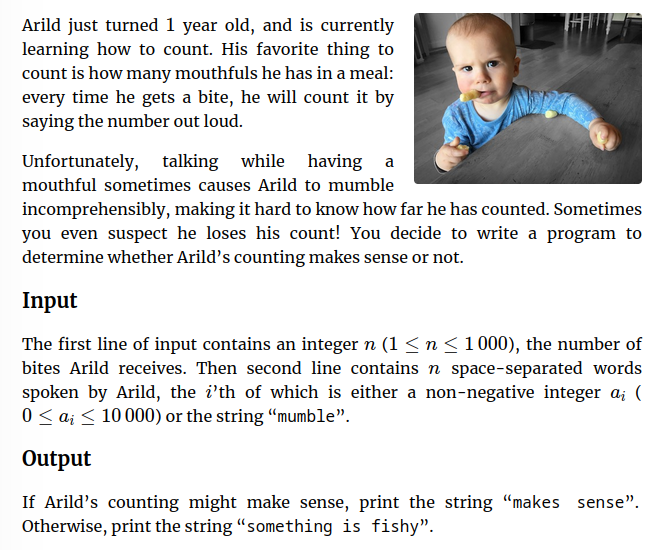
\includegraphics[width=0.9\textwidth]{babybites}
    	\end{center}
\end{frame}

\begin{frame}[plain, fragile]
    \frametitle{Solution}
    \begin{minted}{python}
n = int(input())
words = input().split()
valid = True

for i in range(n):
    if words[i] != "mumble" and l[i] != str(i + 1):
        valid = False
        break

if valid:
    print("makes sense")
else:
    print("something is fishy")
    \end{minted}
\end{frame}

\end{document}

